

% Qué tipo de documento estamos por comenzar:
\documentclass[a4paper]{article}
% Esto es para que el LaTeX sepa que el texto está en español:
\usepackage[spanish]{babel}
\selectlanguage{spanish}
% Esto es para poder escribir acentos directamente:
\usepackage[utf8]{inputenc}
\usepackage[T1]{fontenc}
\usepackage{bold-extra}
\usepackage{graphicx}
\usepackage{subfigure}

%% Asigna un tamaño a la hoja y los márgenes
\usepackage[a4paper,top=3cm,bottom=2cm,left=3cm,right=3cm,marginparwidth=1.75cm]{geometry}

%% Paquetes de la AMS
\usepackage{amsmath, amsthm, amsfonts}
%% Para añadir archivos con extensión pdf, jpg, png or tif
\usepackage{graphicx}
\usepackage[colorinlistoftodos]{todonotes}
\usepackage[colorlinks=true, allcolors=blue]{hyperref}

\newcommand\tab[1][0.5cm]{\hspace*{#1}}

\title{Implementación de un Software web que emula el funcionamineto de la estructura de datos R-Tree}
\author{Felipe Moreno-Vera, Solange Ramos-Cooper,  \\
  Alvaro Rojas-Machado, Jefferson Quispe-Pinares\\
  \small Universidad Católica San Pablo\\
  \small \{felipe.moreno, solange.ramos, luis.rojas, jefferson.quispe\}@ucsp.edu.pe\\
  \small Arequipa,Perú
  \date{15 de agosto de 2018}
}

\begin{document}
\maketitle

 
\begin{abstract}
El área de estudios de estructura de datos multidimensionales, tiene comunmente aplicaciones en Base de Datos o simulaciones de superficies, imágenes o incluso en modelamiento y solución de ecuaciones para encontrar conjuntos de superficies con características específicas.
En el presente proyecto se llevó a cabo el desarrollo de una interfaz web que mediante una adecuada comunicación con un programa núcleo en C++ permite emular mediante inserción de puntos y polígonos así como también la busqueda por area y vecinos más cercanos de una estructura R-Tree, el cual permite poder entender mejor el comportamiento de esta estructura de datos basada en Arboles B.

\end{abstract}

%% Iniciamos "secciones" que servirán como subtítulos
%% Nota que hay otra manera de añadir acentos

\section{Descripción}

Para el proyecto se diseño una interfaz con dos secciones principales como se muestra en la figura \ref{interface}, situando en el lado izquierdo una sección para visualización de elementos y resultados mientras en el lado derecho se encuentra una sección con todas las opciones disponibles por la implementación final.\\

\begin{figure}[htbp]
  \begin{minipage}{.5\linewidth}
  \subfigure[]{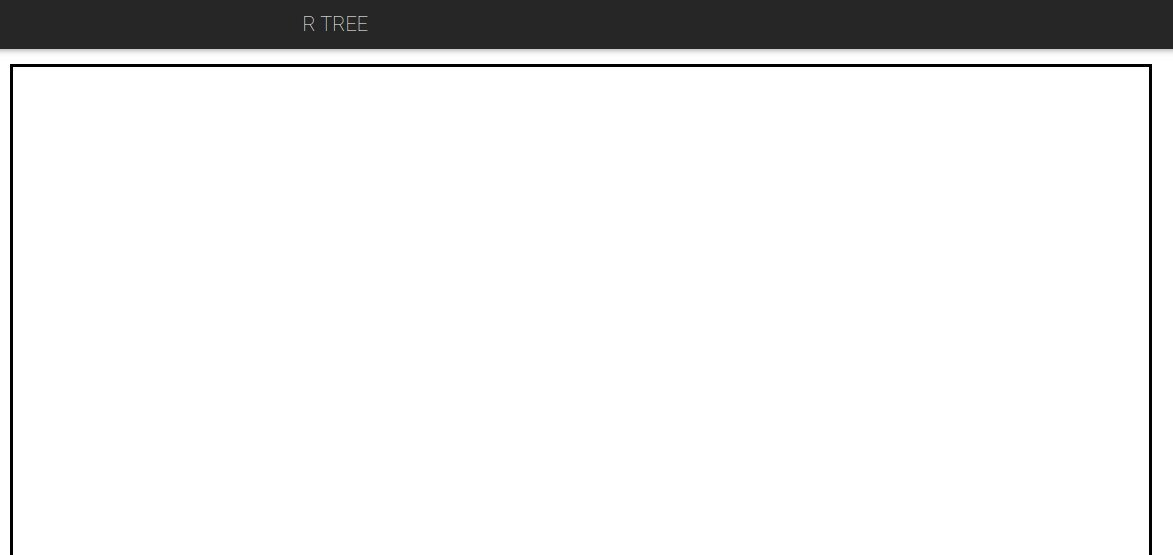
\includegraphics[width=9cm,height=5cm]{images/Interface.jpg}}
  \end{minipage}
  \begin{minipage}{.5\linewidth}
  \subfigure[]{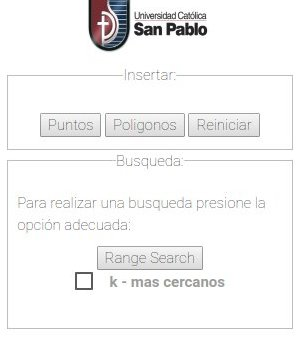
\includegraphics[width=4cm,height=5cm]{images/options.jpg}}
  \end{minipage}
  \caption{(a) Visualización y (b) opciones disponibles en aplicación final.}
\label{interface}
\end{figure}

De la imagen anterior pude visualizarse que las opciones disponibles están divididas en dos grupos, colocando en la parte superior las opciones relacionadas a la inserción y en la inferior las opciones relacionadas a búsqueda de elementos.\\
Entre las opciones de inserción se encuentran las opciones para el ingreso de puntos y polígonos, los cuales deben ser ingresados uno a la vez. Cabe mencionar la presencia del boton \texttt{REINICIAR} para eliminar el árbol existente y al mismo tiempo limpiar la interfaz de visualización.\\
Entre las opciones de búsqueda se encuentran las opciones correspondientes a búsqueda por rango y por cercanía, los cuales al ejecutar las funciones correspondientes cambian el color de los elementos obtenidos.\\

\subsection{R-Tree e implementación del CORE}

R-tree es una estructura de datos basada en los árboles de tipo B, definiendo el número de hijos por nodo entre un valor máximo y uno mínimo. La particularidad del R-Tree es que permite la inserción de data multidimensional en el árbol balanceado.\\

Se logra mantener el árbol balanceado al realizar una inserción directa de los elementos sobre los nodos hojas, eligiendo el nodo adecuado mediante un algoritmo de inserción, el cual asimismo asegura el número máximo de elementos permitidos por nodo separando los elementos en dos nuevos nodos (\texttt{split}) y creando un nuevo elemento adicional en la capa superior.\\

El proceso de \texttt{split} se realiza para cada nivel en el cual sea requerido, incluyendo el nodo raíz en el cual el \texttt{split} divide sus elementos en dos nodos y genera un nuevo nodo padre (nueva raíz).\\
La implementación del algoritmo fue basada en una versión existente realizada por Yariv Barkan\cite{r-tree}, haciendo una adaptación para la correcta comunicación con la interfaz web.\\ 

Estas actualizaciones comienzan con la creación de la función \texttt{UPDATETREE} para actualizar y leer la información del árbol con cada elemento insertado, preparando además la información requerida por la interfaz web para la visualización de los mínimos rectángulos delimitadores (\texttt{MBRs}) del árbol.\\

Asimismo se realizaron modificaciones en las funciones \texttt{INSERT}, \texttt{SEARCH} y funciones asociadas para cumplir con especificaciones de la aplicación desarrollada además de la creación de funciones adicionales. Otra actualización importante es la implementación del algoritmo de búsqueda \texttt{k-Nearest Neighbor} para la localización de los k elementos más cercanos a un punto especificado en el programa.\\

Esto en conjunto con el desarrollo de la interfaz web y programa para la interconexión permite el correcto funcionamiento de la aplicación web desarrollada.

\subsubsection{Descripción de la estructura de datos} % solange o alvaro
El programa general se basa en el diseño de la clase RTree que posee funciones y objetos asociados entre los cuales se encuentran los nodos, elementos en nodos y \texttt{MBRs}. En forma general se puede decir que cada nodo contiene un número limitado de elementos denominados en el programa como \texttt{branch}, este número es maximo 4 y minimo 2. Al mismo tiempo cada \texttt{branch} tiene asociado un \texttt{MBR} y un nodo hijo, siendo que en los nodos hojas los \texttt{branchs} corresponden a los objetos insertados y sus hijos son nodos NULL. Por defecto se inicializa el nodo raíz con 0 elementos.\\

\subsubsection{Implementación de la función \texttt{INSERT}} % solange o alvaro

La función \texttt{INSERT} es la encargada de colocar los nuevos elementos en el árbol, ubicándolos como hojas y realizando \texttt{splits} en los \texttt{MBRs} en caso se requiera. Para lograr esto la función usada tiene como entradas los limites máximos y mínimos del elemento por cada dimensión, colocando además una ID asociada al elemento según el orden en el que sea ingresado.\\

La función \texttt{INSERT} tras corroborar que los límites mínimos ingresados sean menores a los máximos crea un nuevo \texttt{Branch} a la cual asocia la ID ingresada, límites ingresados e hijos \texttt{NULL}. Resumidamente esta función verifica la validez de los datos a ingresar, crea un nuevo \texttt{branch} y llama a la función \texttt{INSERTRECT}.\\

%\textbf{Datos de entrada:}
%\begin{itemize}
  %  \item \texttt{min[]}: Límites inferiores por dimensión.
 %   \item \texttt{max[]}: Límites superiores por dimensión.
%    \item \texttt{ID\_elemento}: Orden de ingreso del elemento ya sea punto o polígono. 
%\end{itemize}

%\texttt{\textit{Insert(min[],max[], ID\_elemento)}}\\
%\tab \texttt{\textit{Crear nuevo Branch}}\\
%\tab \texttt{\textit{En estructura Branch definir elemento ID como ID\_elemento}}\\
%\tab \texttt{\textit{En estructura Branch definir elemento nodo como NULL}}\\
%\tab \texttt{\textit{Llamar a función INSERTRECT}}\\

La función \texttt{INSERTRECT} recibe como entrada el nuevo branch creado, la raíz del árbol y un nivel de hojas declarado como 0. Esta función llama a la función recursiva con retorno booleano \texttt{INSERTRECREC}, la cual indica en su salida si es requerido un \texttt{split}. Al terminar los llamados a la función recursiva se verifica si es necesario un \texttt{split} en la raíz, según lo cual la función \texttt{INSERTRECT} realiza un \texttt{split} especial generando un nuevo nodo raíz, al cual le asigna el nivel correspondiente y lo asigna como nodo raíz. Se procede a mostrar el pseudocódigo de las funciones \texttt{INSERTRECT}.\\
\textbf{Datos de entrada:}
\begin{itemize}
    \item \texttt{Branch}: Branch creado en la función \texttt{INSERT}.
    \item \texttt{m\_root}: Nodo raíz del árbol.
\end{itemize}

\texttt{\textit{Insertrect(Branch, m\_root)}}\\
\tab \texttt{llamar a función recursiva \textit{INSERTRECTREC}}\\
\tab \texttt{\textit{Si} se requiere split en m\_root}\\
\tab \tab \texttt{Realizar split en m\_root}\\
\tab \tab \texttt{Crear nuevo nodo Raíz}\\

La función recursiva \texttt{INSERTRECTREC} mencionada anteriormente es aquella encargada de elegir el \texttt{branch} adecuado en el nodo, llamando de forma recursiva sobre el nodo correspondiente al \texttt{branch} elegido. Esta llamada recursiva se realiza hasta llegar a las hojas donde inserta directamente el elemento. Tras ejecutarse las llamadas recursivas la función realiza la expansión de los \texttt{MBRs}, la verificación del número de \texttt{branch} por nodo y en caso sea necesario los \texttt{splits} y creación de nuevos \texttt{branch} requeridos. A continuación se describe el pseudocódigo y luego a más detalle el funcionamiento de \texttt{INSERTRECTREC}:\\

\textbf{Datos de entrada:}
\begin{itemize}
    \item \texttt{Node}: Nodo de análisis, el primer nodo en análisis es la raíz.
    \item \texttt{Branch}: Branch creado al inicio de la función \texttt{INSERT}.
\end{itemize}

\texttt{\textit{Insertrectrec(Node, Branch)}}\\
\tab \texttt{\textit{Si} es nodo interno}\\
\tab \tab \texttt{Elegir Brunch adecuado con función \textit{PickBranch}}\\
\tab \tab \texttt{Realizar llamada recursiva.}\\
\tab \tab \texttt{\textit{Si no} requiere Split}\\
\tab \tab \tab \texttt{Actualizar MBR}\\
\tab \tab \texttt{\textit{Si} requiere Split}\\
\tab \tab \tab \texttt{Realizar split y agregar nuevo elemento en nodo padre con la funcion \textit{ADDBRANCH}}\\
\tab \texttt{\textit{Si} es nodo hoja}\\
\tab \tab \texttt{Insertar directamente con función \textit{ADDBRANCH}}\\

Para elegir el \texttt{branch} sobre el cual realizar la llamada recursiva se utiliza la función \texttt{PICKBRANCH}, la cual comprueba en los \texttt{MBRs} correspondientes a cada \texttt{branch} del nodo la elongación requerida para contener al nuevo elemento retornando aquel \texttt{branch} cuyo \texttt{MBR} requiere menor elongación. En caso existan múltiples \texttt{MBRs} con la misma elongación requerida se procede a elegir aquel con menor área. Se realiza esta llamada recursiva hasta llegar a un nodo de nivel 1, el cual contiene directamente elementos hoja del árbol. A continuación se muestra el pseudocódigo de la función \textit{PICKBRANCH}:\\

\textbf{Datos de entrada:}
\begin{itemize}
    \item \texttt{Node}: Nodo de análisis, el primer nodo en análisis es la raíz.
    \item \texttt{rect}: MBR del Branch creado al inicio de la función \texttt{INSERT}.
\end{itemize}

\texttt{\textit{PickBranch(Node, Rect)}}\\
\tab \texttt{\textit{Para cada branch del nodo}}\\
\tab \tab \texttt{Retornar indice de branch con MBR con mínima elongación requerida para que contenga a rect.}\\
\tab \tab \texttt{\textit{Si} hay múltiples MBR con igual elongación requerida}\\
\tab \tab \tab \texttt{Retornar índice branch que tenga MBR con menor área}\\

La función \texttt{INSERTRECTREC} al pasar la llamada recursiva al ejecutarse sobre los nodos cuyos hijos son hojas llama directamente a la función \texttt{ADDBRANCH}, la cual agrega el \texttt{branch} creado inicialmente al nodo o llama a la función \texttt{split} en caso el número de elementos en el nodo lo requiera. Ahora procedemos a mostrar el pseudocódigo de la función \texttt{split} y posteriormente explicar algo más su funcionamiento:\\

\textbf{Datos de entrada:}
\begin{itemize}
    \item \texttt{Node}: Nodo sobre el cual se realizará el split.
\end{itemize}

\texttt{\textit{Split(Node)}}\\
\tab \tab \texttt{Inicializar dos nodos con los dos branchs que requieran el MBR más grande para contenerlos.}\\
\tab \tab \texttt{textit{Para cada elemento del nodo restante}}\\
\tab \tab \tab \texttt{Insertar en el nodo correspondiente al MBR que requiera menor elongación para contenerlo.}\\

Para realizar el \texttt{split} se inicializan dos grupos usando los elementos que para ser englobados requieren el rectangulo con mayor área. Tras eso cada elemento se agrega al grupo que requiera menor expansión, hasta que llegue al máximo número de elementos por nodo.\\

Por otra parte si la función \texttt{INSERTRECTREC} se ejecuta sobre nodos con hijos no hojas al pasar la llamada recursiva usa un condicional basado en el retorno de la anterior llamada recursiva. Si este retorno indica que no se requiere un \texttt{split} solo actualiza los \texttt{MBRs} correspondientes de modo que contengan los nuevos hijos que fueron agregados (hojas) o modificados (\texttt{MBRs}). En caso se requiera un \texttt{split} sobre nodos con hijos no hojas este \texttt{split} separará los \texttt{MBRs} asociados a los hijos.

\subsubsection{Implementación de la función  \texttt{SEARCH}} % solange o alvaro
En la función \texttt{SEARCH} se determinan todos los objetos que se encuentren dentro de la región ingresada por el usuario. Si no existen coincidencias, devuelve un conjunto vacío. En este caso se tomó en cuenta solo los objetos cuyos \texttt{MBR} se encuentren completamente cubiertos por la región de consulta. La función  \texttt{SEARCH} hace un llamado a una segunda función  \texttt{SEARCH} para iniciar la búsqueda en el nodo raíz, luego esta función realiza un llamado recursivo hasta llegar a los nodos hoja del árbol. En esta función se almacenarán la cantidad de elementos que son cubiertos por la región de consulta.\\

En la función \texttt{SEARCH}, para el \texttt{nodo} actual se verifica si este es interno o no. Si es nodo interno, para cada una de las entradas del nodo se verifica si el \texttt{MBR} sobrepone de dicha entrada se sobrepone a la región de consulta, si fuera así, se llama a la función \texttt{SEARCH} con el nodo hijo asociado a la entrada del elemento actual.
Si el \texttt{nodo} actual es nodo hoja, para cada entrada en el nodo (en este caso cada entrada representa un objeto dato) se verifica si la región de consulta cubre por completo el \texttt{MBR} de la entrada actual, si es así, se incrementa un contador, el identificador del objeto actual es agregado a una lista, y luego se continúa con la búsqueda. El pseudocódigo de la segunda función \texttt{SEARCH} se puede ver a continuación.\\

\textbf{Datos de entrada:}
\begin{itemize}
    \item \texttt{nodo}: Nodo actual en el cual se hará la búsqueda, puede ser nodo hoja o nodo interno.
    \item \texttt{region\_consulta}: Región de consulta ingresado por el usuario.
    \item \texttt{cantidad\_encontrados}: Cantidad de elementos encontrados dentro de la región consulta 
\end{itemize}

\texttt{\textit{Search(nodo, region\_consulta, cantidad\_encontrados)}}\\
\tab \texttt{\textit{Si } \textit{nodo} actual NO es nodo hoja }\\
\tab \tab \texttt{\textit{Para cada} entrada en el nodo actual}\\
\tab \tab\tab \texttt{\textit{Si } MBR de la entrada actual se sobrepone a la \textit{region\_consulta}}\\
\tab \tab\tab\tab \texttt{ \textit{Search(nodo hijo del elemento, region\_consulta, cantidad\_encontrados)}}\\
\tab \texttt{\textit{Sino}} \\
\tab \tab \texttt{\textit{Para cada} entrada en el \textit{nodo}}\\
\tab \tab\tab \texttt{\textit{Si } MBR de la entrada actual cubre por completo a la \textit{región\_consulta}}\\
\tab \tab\tab\tab \texttt{Incrementar contador y agregar identificador de objeto a la lista}\\

\subsubsection{Implementación de la función \texttt{SEARCH\_KNN}} % solange o alvaro
En la función \texttt{SEARCH\_KNN} se determinan los \texttt{K} elementos más cercanos a un punto determinado por el usuario. En este caso se tomó en cuenta la distancia Euclideana entre los \texttt{MBR} de los objetos almacenados y el punto de consulta. La función  \texttt{SEARCH\_KNN} hace un primer llamado a la función  \texttt{SEARCH\_NN} para iniciar la búsqueda en el nodo raíz, luego esta función realiza un llamado recursivo hasta llegar a los nodos hoja del árbol. En esta función se almacenarán los \texttt{K} elementos más cercanos, se crea una lista inicial de \texttt{k} elementos con  distancias máximas. \cite{Kuan} \cite{Cheung} \\

En la función \texttt{SEARCH\_NN}, para el \texttt{nodo} actual se verifica si este es interno o no. Si es nodo interno, se crea una lista temporal de todas las entradas que pertenecen al actual \texttt{nodo}, almacenando la distancia entre los  \texttt{MBR} de cada entrada y el \texttt{punto\_consulta}. Luego, se ordenan ascendentemente los objetos de la lista según la distancia. Esto se hace con la finalidad de priorizar y acceder a los nodos hijos cercanos antes que a los lejanos. Luego, por cada elemento en la lista temporal se verifica si la distancia en el actual elemento es menor que la distancia del k-ésimo elemento en la lista los \texttt{k\_cercanos }, si fuera así, se llama a la función \texttt{SEARCH\_NN} con el nodo hijo asociado al elemento actual en la lista temporal. \\

Si el \texttt{nodo} actual es nodo hoja, para cada entrada en el nodo (en este caso cada entrada representa un objeto dato) se calcula la distancia entre el objeto y el \texttt{punto\_consulta}. Luego se verifica si esta distancia es menor que la distancia del k-ésimo elemento en la lista los \texttt{k\_cercanos }, si fuera así, este objeto es agregado a la lista  \texttt{k\_cercanos }. El pseudocódigo de la función \texttt{SEARCH\_NN} se puede ver a continuación.\\

\textbf{Datos de entrada:}
\begin{itemize}
    \item \texttt{punto\_consulta}: Punto de consulta ingresado por el usuario.
    \item \texttt{nodo}: Nodo actual en el cual se hará la búsqueda, puede ser nodo hoja o nodo interno.
    \item \texttt{k\_cercanos}: Lista de los $k$ elementos más cercanos ordenada de acuerdo a la distancia calculada entre el elemento y el punto de consulta.
    \item \texttt{k}: Cantidad de elementos más cercanos. También ingresado por el usuario.\\
\end{itemize}

\texttt{\textit{Search\_nn(punto\_consulta, nodo, k\_cercanos, k)}}\\
\tab \texttt{\textit{Si } \textit{nodo} actual NO es nodo hoja }\\
\tab \tab \texttt{Generar una lista temporal con todas las entradas del \textit{nodo}}\\
\tab \tab \texttt{Ordenar lista ascendentemente según distancia}\\
\tab \tab \texttt{\textit{Para cada} elemento en la lista temporal}\\
\tab \tab\tab \texttt{\textit{Si } distancia del actual elemento  $ < $  distancia \textit{k\_cercanos[k-1]} elemento}\\
\tab \tab\tab\tab \texttt{Search\_nn(\textit{punto\_consulta}, nodo hijo del elemento, \textit{k\_cercanos}, \textit{k)} }\\
\tab \texttt{\textit{Sino}} \\
\tab \tab \texttt{\textit{Para cada} entrada en el \textit{nodo}}\\
\tab \tab\tab \texttt{Calcular distancia entre objeto y \textit{punto\_consulta}}\\
\tab \tab\tab \texttt{\textit{Si } distancia calculada $ < $ distancia \textit{k\_cercanos[k-1]} elemento }\\
\tab \tab\tab\tab \texttt{Agregar elemento a \textit{k\_cercanos }}\\

\subsection{Implementación de la conexión entre el programa R-Tree y el servicio web} % felipe

En esta sección se presenta la interconexión usnado MQTT entre el R-Tree desarrollado en C++ y la interface web hecha en js y html con un servicio en go.

\subsubsection{Message Queuing Telemetry Transport}

El protocolo de comunicación utilizado es MQTT (Message Queue Telemetry Transport) \cite{mqtt} el cual es un protocolo de bajo consumo de energía y bajo consumo de recursos (a nivel de transferencia y envío de datos) el cual trabaja bajo el modelo de \textbf{Subscriptor - Publicador}.

\begin{figure}[ht]
\centering
  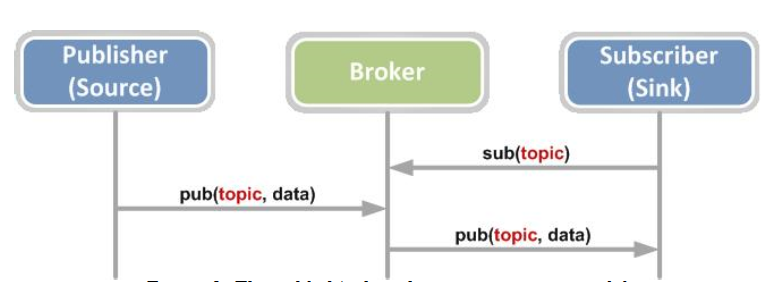
\includegraphics[width=10.5cm]{images/model.png}
  \caption{MQTT model}
  \label{fig1}
\end{figure}

Es decir, se tiene un servicio llamado mosquitto (o mosca en Python) el cuál esta a la escucha de intercambio de mensajes por parte de los clientes que publican o se suscriben, a los tag de subscripción se les denomina \textbf{Tópicos}.

Se instaló el servicio mosquitto (mqtt) hecho en c++ y también las librerías para los respectivos lenguajes, la librería Paho.mqtt.client \cite{paho} provee lo necesario para poder implementar clientes a nivel web (a través de websockets) y clientes como dispositivos (consola o cualquier sistema) a través de sockets. Para la parte del sistema o consola, se uso el cliente C++ y para la parte web, el cliente Javascript.

\begin{figure}[ht]
\centering
  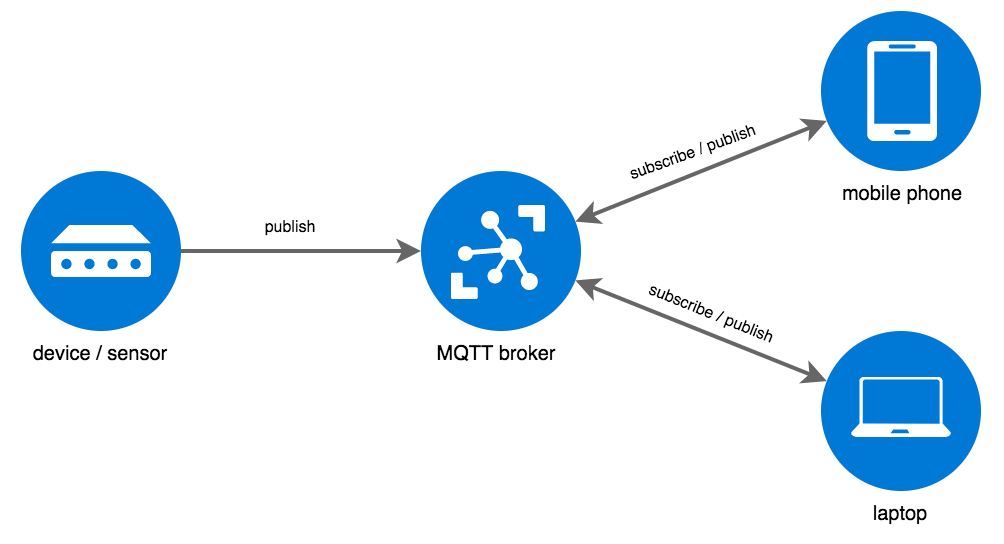
\includegraphics[width=8.5cm]{images/broker.png}
  \caption{MQTT model}
  \label{fig2}
\end{figure}

Para tener el servicio mosquitto activo, se debe instalar en el sistema operativo y luego configurar el fichero \textit{mosquitto.conf}, se debe añadir los protocolos y numero de puertos como 1883 para dispositivos y 1884 para websockets.

En el fichero mencionado, se pueden realizar configuraciones como máximo numero de conexiones o restringir accesos, el servicio web fue implementado en el lenguaje de programación Go en el puerto 80, el cual es consumido por los clientes web. Además, permite la conexión vía WebSocket del cliente web MQTT.

El protocol MQTT a diferencia de HTTP o sockets, segura que el mensaje llegue a su destino así se pierda la conexión debido a que permite definir un buffer máximo de tamaño variable que contiene los últimos mensaje de texto enviado. Esta demás decir que apicaciones como whatsapp y fb-messenger utilizan este protocolo.

Lea el \textit{Readme.md} o la referencia de instalar \cite{jenazads} para más detalle.

\subsection{Implementación de la interfaz web} % jefrey
Para la implementación web el objetivo es generar una experiencia agrable al usuario cuya percepción sea positiva con la aplicación. En nuestro caso y como habitualmente en el mundo del desarrollo web, nuestra parte del cliente esta desarrollada en CSS, Javascrypt y html5, además de estas usamos de manera adicional la librería de javascript con la nomenclatura de Fabric.js, framework Materialize y Jquery que nos proporciona herramientas ideales para una exitosa interacción con el usuario.
\subsubsection{Canvas (Html)}
Para los dibujos usamos Canvas, es un elemento de html5 que permite la generación de gráficos dinámicamente por medio de scripting.Entre otras cosas, permite la renderización  dinámica de gráficos 2D y mapas de bits, así como animaciones con estos gráficos. Se trata de un modelo de procedimiento de bajo nivel, que actualiza un mapa de bits y no tiene una gráfica de escena integrada.
Hemos definido dentro de nuestro propio Canvas una dimensión de 800x600 (altura y anchura), dentro de la región nuestras funciones y eventos interactuaran en ella. 

\subsubsection{Libreria Fabric.js}
Fabric.js es una poderosa y simple librería de Javascrip y Html con Canvas, esta  provee de un modelo de objeto interactivo sobre el elemento  Canvas. También tiene una analizadores SVG a Canvas y viceversa. 
En nuestra aplicación usamos los objetos geométricos como punto, círculo, línea, rectángulo y la construcción de polígono en bases de los elementos anteriores, la edición de estas figuras geométricas depende de los valores de entrada que deseemos ingresar, la respuesta del core de Rtree sera inmediata a través de los datos de salida que sera dibujado dentro de nuestro Canvas.
\subsubsection{Framework Materialize}
Es un moderno framework CSS basada en Material Design, dentro de sus características esenciales obtenidas para nuestro proyecto es la técnica estética de estilos que posee para mostrar una interfaz amigable e intuitiva, posee un diseño web responsive que permite la visualización correcta en dispositivos de cualquier tamaño. Nuestro comando de "Insertar" y de "Búsqueda" posee los estilos de este framework.

\section{Resultados}

\subsubsection{R-Tree}
En esta sección se hizo una prueba de estress insertando, buscando (por area y knn) desde 1000 hasta 9000 elementos (no se pudo probar 10000 debido a que la máquina en la que se hizo las pruebas no soportó), todas estas pruebas estan en el fichero \textbf{Test.cpp}.

\begin{itemize}
    \item \textbf{Insertar} Inserta elementos  de puntos aleatorios
    
    \begin{tabular}{ |p{3cm}||p{3cm}|p{3cm}|p{3cm}|  }
     \hline
     num data & time\\
     \hline
     1000 & 0.068553  \\
     2000 & 0.136289  \\
     3000 & 0.276568  \\
     4000 & 0.484284  \\
     5000 & 0.868381  \\
     6000 & 1.2564  \\
     7000 & 1.13003  \\
     8000 & 2.27265  \\
     9000 & 1.8945  \\
     \hline
    \end{tabular}
    
    \item \textbf{Buscar por Area} Busca en regiones de puntos aleatorios
    
    \begin{tabular}{ |p{3cm}||p{3cm}|p{3cm}|p{3cm}|  }
     \hline
     num data & time\\
     \hline
     1000 & 0.028233  \\
     2000 & 0.112528  \\
     3000 & 0.254016  \\
     4000 & 0.48334  \\
     5000 & 0.732972  \\
     6000 & 1.00877  \\
     7000 & 1.37457  \\
     8000 & 1.74464  \\
     9000 & 2.20014  \\
     \hline
    \end{tabular}
    
    
    \item \textbf{Buscar Knn} Busca knn vecinos cercanos para k = 100
    
    \begin{tabular}{ |p{3cm}||p{3cm}|p{3cm}|p{3cm}|  }
     \hline
     num data & time\\
     \hline
     1000 & 0.144627  \\
     2000 & 0.357828  \\
     3000 & 0.529841  \\
     4000 & 0.847712  \\
     5000 & 1.12524  \\
     6000 & 0.854988  \\
     7000 & 1.18532  \\
     8000 & 1.48988  \\
     9000 & 1.65935  \\
     \hline
    \end{tabular}
\end{itemize}

\subsection{Modo Inserción}
Este modo permite ingresar elementos en el árbol, los elementos pueden ser puntos o polígonos. Los elementos son enviados al programa núcleo donde son tratados como dos arreglos de puntos (máximos y mínimos). Estos puntos también se ven reflejados en el Canvas como los \texttt{MBR} formados por el algoritmo y los \texttt{split} respectivos dado las condiciones iniciales: Máxima cantidad de elementos por nodo $M=4$, y mínima cantidad de elementos por nodo $m=2$.   
\begin{figure}[ht]
\centering
  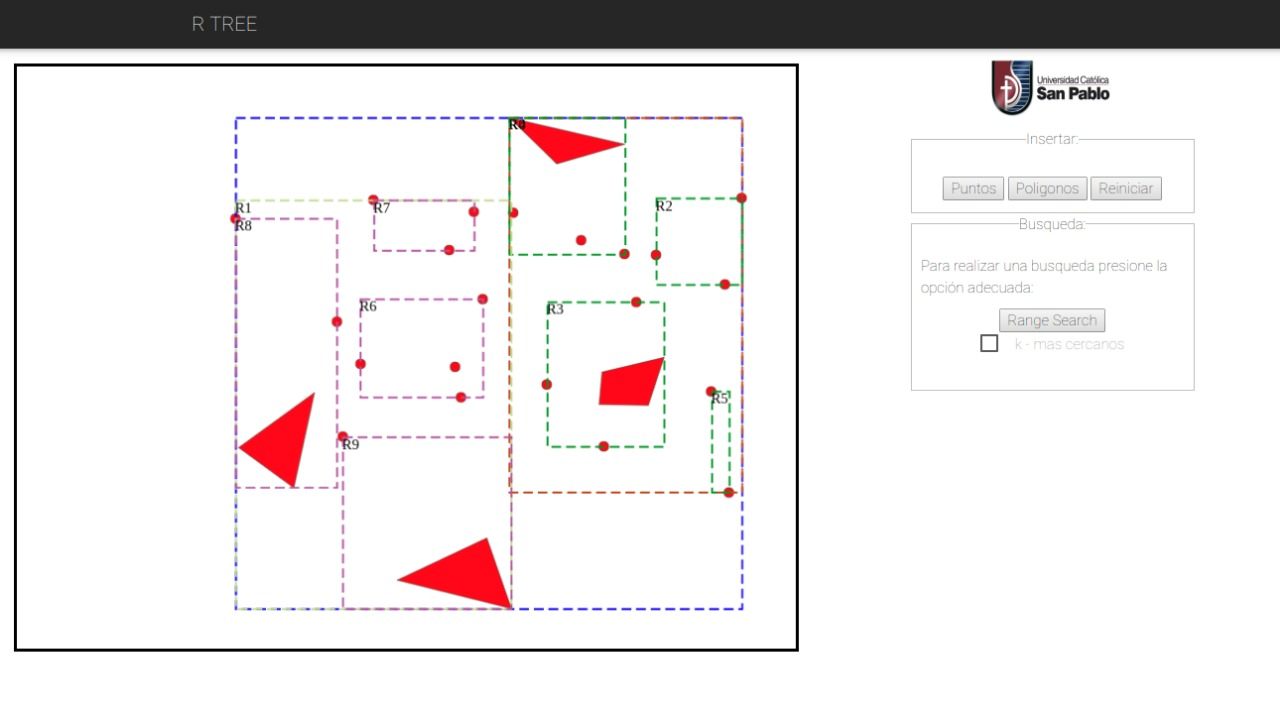
\includegraphics[width=10.5cm]{images/insert.jpeg}
  \caption{Insert Polígonos y Puntos}
  \label{fig3}
\end{figure}
\subsection{Modo Consulta}
Este modo permite realizar consultas de búsqueda de dos tipos. El primero es de tipo \texttt{Range Query} (\textit{Figura 5}), el cuál retorna los elementos que se encuentran dentro de una región definida por el usuario, los elementos son pintados de un mismo color en el canvas. El segundo es de tipo \texttt{K-Nearest Neighbor} (\textit{Figura 6}), esta consulta retorna los $k$ elementos más cercanos a un punto definido por el usuario, estos elementos son pintados de un mismo color en el canvas, así como también se traza una linea desde el punto consulta hacia cada elemento encontrado. El número de elementos $k$ también es ingresado por el usuario. 
\begin{figure}[ht]
\centering
  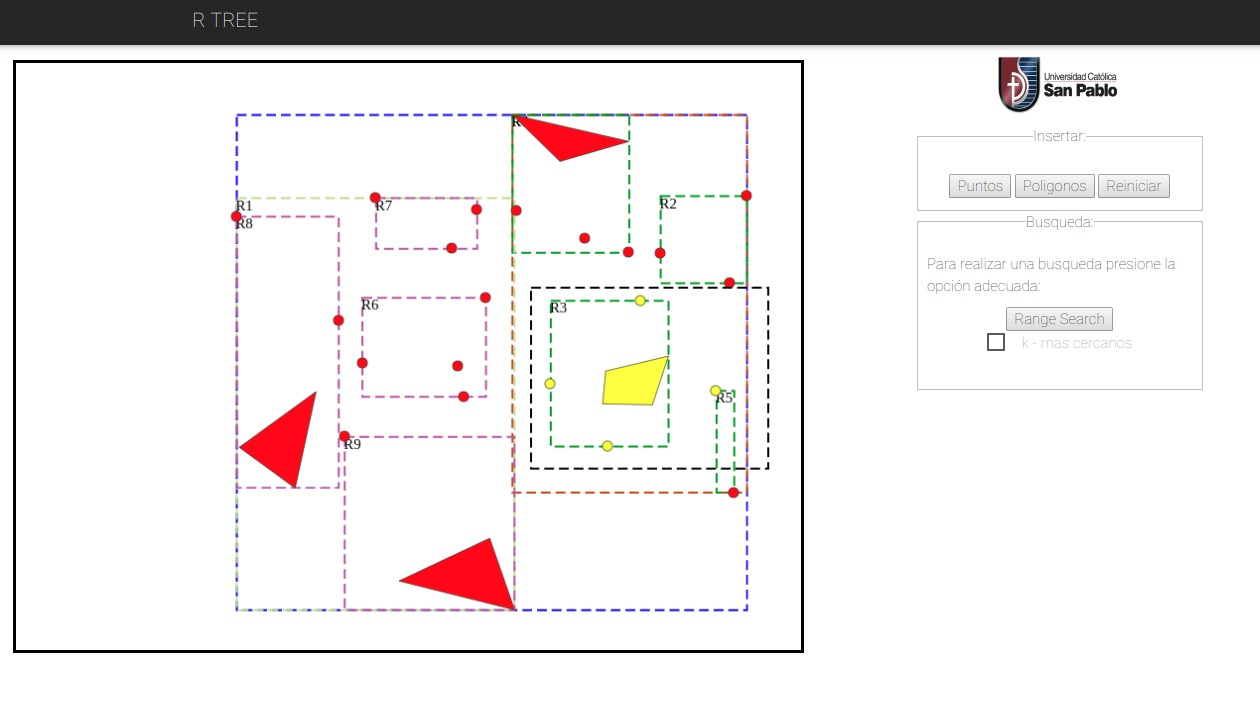
\includegraphics[width=10.5cm]{images/search.jpeg}
  \caption{Range Query}
  \label{fig4}
\end{figure}

\begin{figure}[ht]
\centering
  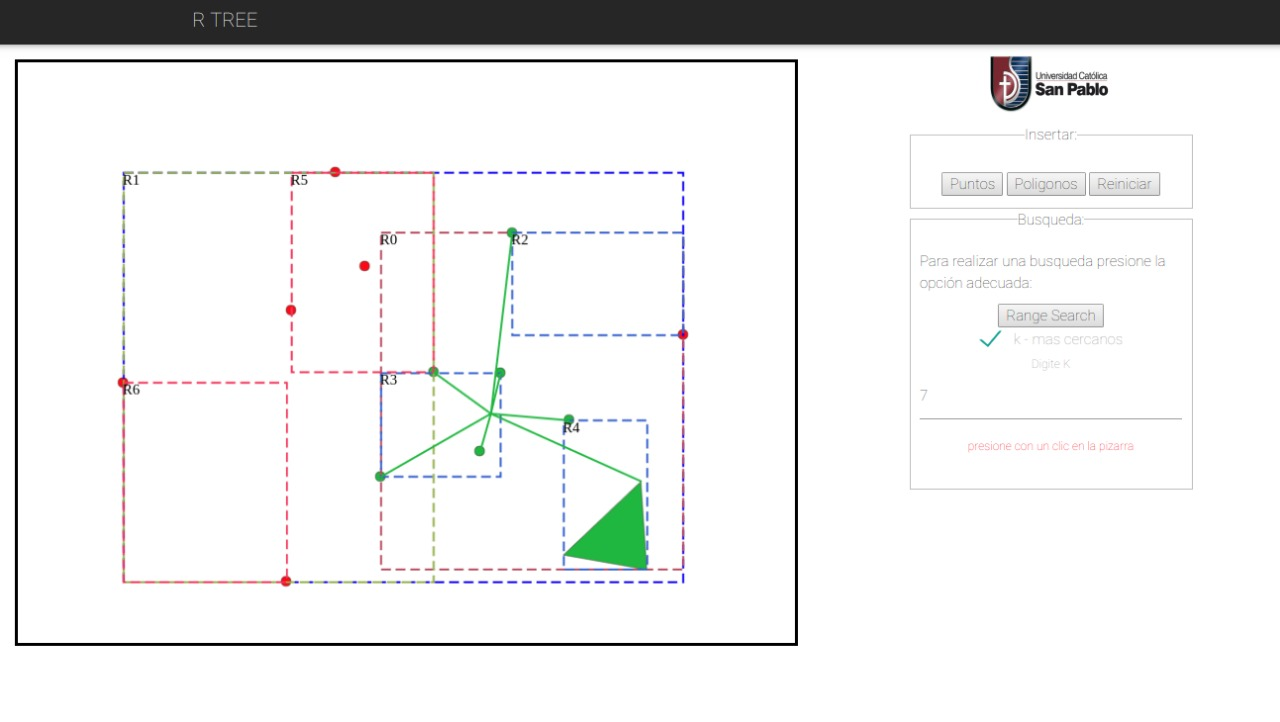
\includegraphics[width=10.5cm]{images/KNEAR.jpeg}
  \caption{K-Nearest Neighbor Query}
  \label{fig5}
\end{figure}

\newpage

\section{Limitaciones}
A continuación se mencionarán algunas limitación del presente trabajo.\\
\begin{itemize}
    \item Existen diversas librerías y frameworks, por lo tanto se posee la dificultad temporal para poder encontrar herramientas que se puedan integrar fácilmente si no existe alguna experiencia previa en desarrollo de estas.
\end{itemize}

\begin{itemize}
    \item Dado que los elementos que son almacenados en nuestra estructura de datos son de tipo bidimensional; es decir, que podrían representar ubicaciones o diferentes espacios sobre un área, no se validó el tema de sobre posición de elementos. Por lo tanto, la plataforma web permite dibujar $n$ polígonos sobre una misma área.
\end{itemize}
\section{Trabajos futuros}

Este proyecto se puede reutilizar para implementar derivados o estructura de datos similares.

En el actual trabajo el tipo de split implementado es Cuadrático,  se tiene proyectado la implementación de distintos tipos de split  como el R-Star y lineal para verificar el rendimiento de estas, esta experimentación nos permitirá concluir el split adecuado para algún caso particular.

Con el presente proyecto establecemos el punto de partida  para desarrollar las aplicaciones orientadas a la vida real que nos permite usarlo en distintos ámbitos de Sistemas de Información Geográfica (GIS) incluyendo datos geográficos.

\section{Conclusiones}

En el presente trabajo se busca simular el funcionamiento de la estructura de datos R-Tree, la cual almacena elementos de n-dimensiones en sus nodos hoja, y e los demás nodos hace referencia a regiones contenedoras de dichos elementos. 

Además se presenta una manera en como realizar una comunicación bi-direccional entre una interfaz web (levantada en un servicio web) con un programa de lenguaje compilado como cpp, los cuales se comunican a través de mensajería de texto (formato JSON).

Se propuso el protocolo de comunicacón MQTT en vez de sockets nativos o HTTP debido a que MQTT es un protocolo diseñado para consumir los mínimos recursos en conexión de redes lentas o de muy baja latencia, asegurando que el mensaje llegue a su destino.

Se utilizó el servicio AWS para que se pueda acceder al servicio desde cualquier lugar (a través de un navegador web).

\section{Distribución del trabajo}
Para el desarrollo del presente proyecto, las tareas fueron divididas entre todos los colaboradores de la siguiente manera:
\begin{itemize}
    \item \textbf{R-Tree} La implementación del R-Tree abarca desde el diseño de la estructura de datos (nodo, clase árbol, templates y funciones insert, update, remove, removeAll, add y count) incluyendo la búsqueda por rango o \textit{Range Search} y la búsqueda de los K vecinos más cercanos o \textit{K-Nearest-Neighbours}, estuvo a cargo de Alvaro Rojas y Solange Ramos. 
    \item \textbf{Conexión web service - programa} La implementación, configuración del servicio MQTT con mosquitto, asi como la implementación de los clientes en cpp (socket) y la integración con el programa principal de R-Tree y a integración del cliente js (websocket) con la interfaz web los cuales funcionan para el intercambio de información a través de mensajes en formato JSON, además de la configuración del sericio Web en el lenguaje Go y su configuración en la instancia EC2 en AWS estuvo a cargo de Felipe Moreno.
    \item \textbf{Interfaz Web} El diseño y organización de los componentes visuales de la interfaz web, así como también el uso de librerías para dibujar sobre canvas (abarca desde insertar puntos, polígonos, las funciones range search, knn, los MBR y demás componentes visuales) como fabric.js y además de la funcionalidad de responsive en páginas web estuvo a cargo de Jefferson Quispe.
\end{itemize}

\section{Link repositorio Github}

El link del repositorio es \url{https://github.com/jeffersonquispe/ED2018-MCS}.

\section{Link Video}

El link del video es \url{https://www.youtube.com/watch?v=0jldAnMn3dU}

\section{Link de la simulación web del R-Tree}

El link de la página web que emula el comportamiento del R-Tree es \url{http://r-tree.nezads.com}

\begin{thebibliography}{9}
\bibitem{Kuan} 
J. Kuan and P. Lewis. \textit{Fast k nearest neighbour search for r-tree family} In Information, Communications and Signal Processing, 1997. ICICS.,Proceedings of 1997 International Conference on, pages 924–928 vol.2, 1997.

\bibitem{Cheung} 
K. L. Cheung and A. W.-C. Fu. \textit{Enhanced nearest neighbour search on the R-tree}. SIGMOD Record,
27(3):16–21, 1998.

\bibitem{r-tree}
nushoin, R-Tree, \url{https://github.com/nushoin/RTree}. Last visited 13/08/2018.

\bibitem{mqtt}

MQTT-Org, Protocols, \url{http://mqtt.org/}. Last visited 13/08/2018.

\bibitem{paho}
Paho, Clients, \url{http://www.eclipse.org/paho/clients/cpp/}. Last visited 13/08/2018. 

\bibitem{jenazads}
Felipe A. Moreno, Install Paho Client, \url{https://github.com/Jenazads/PahoMQTTClients}. Last visited 15/08/2018.

\end{thebibliography}

\end{document}